\chapter{Deriving Equations of Motion}

\section{Method for deriving EOMs}

\begin{enumerate}
	\item Assign coordinates by selecting the type of system (Cartesian or polar)
	\item Determine DOF
	\item For each DOF there is a EOM
	\item Determine the accelerations using the standard formulae from either Cartesian or Polar coordinates forms
	\item Draw FBDs
	\item From FBDs we get $\sum F_{ext}$, the $m a_{B/O}$ part is derived from step 4
	\item If there are moments in the system use formulae from angular momentum and torques to construct $\sum \tau = d h_{B} / dt$
\end{enumerate}

\section{Exercise 1}

Consider a system as shown in figure \ref{fig_0_ch_4_exercise1}.
\begin{figure}[h!]
	\centering
	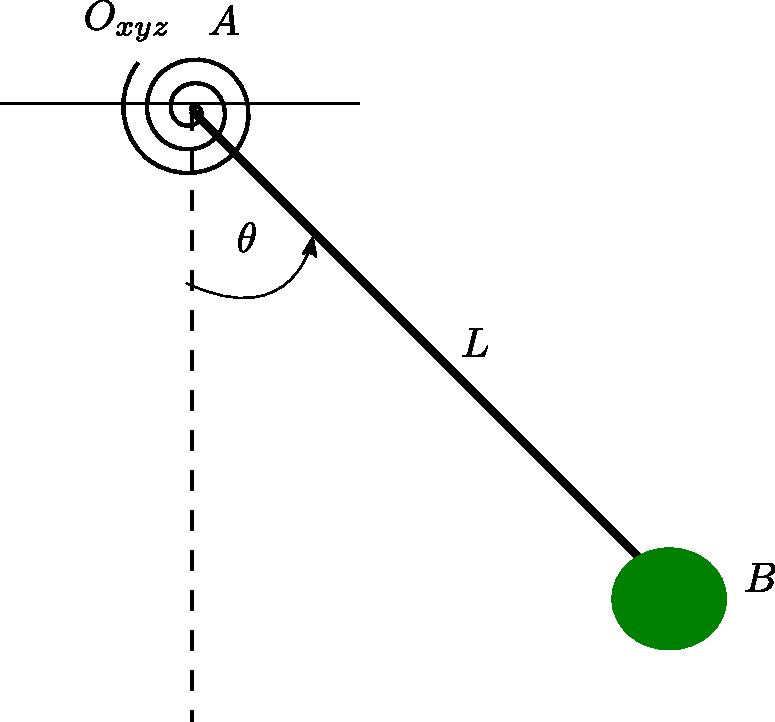
\includegraphics[width=0.5\linewidth]{Bilder/17_PendulumExercise.pdf}
	\caption{Pendulum attached to a torsional spring}
	\label{fig_0_ch_4_exercise1}
\end{figure}

\subsubsection{Assigning coordinates}

Because this is a rotation problem, choosing polar coordinates for this system. Choosing $\hat{r}$ along the length of the pendulum with positive side pointing away from the pendulum, $\hat{\theta}$, positive to CCW direction of pendulums rotation. 

\subsection{DOF}

Constraints on the system:
\begin{enumerate}
	\item $z = \dot{z} = \ddot{z} = 0$
	\item $\dot{r} = \ddot{r} = 0$
\end{enumerate}
there is only one possible motion along $\hat{\theta}$  with the pendulum pivoted to the ceiling, EOM of this problem should be constructed according to
\begin{equation}
	\sum \tau_{ext} = \frac{d}{dt}h_{B/A}
\end{equation}

\subsection{Determine angular momentum the system}

Angular momentum pendulum $B$ pivoted to point $A$ is expressed using equation
\begin{equation}
	h_{B/A} = r_{B/A} \times p_{B/O}
\end{equation}
with $r_{B/A} = L \hat{r}$. Determining $p_{B/O}$:
\begin{equation}
	p_{B/O} = m v_{B/O}
\end{equation}
$v_{B/O}$ in polar coordinates is expressed as
\begin{equation}
	v_{B/O} = \dot{r}\hat{r} + r \dot{\theta} \hat{\theta} = L \dot{\theta}\hat{\theta}
\end{equation}
substituting $v_{B/O}$ in the equation for $p_{B/O}$:
\begin{equation}
	p_{B/O} = m L \dot{\theta}\hat{\theta}
\end{equation}
finally, substituting $p_{B/O}$ into the equation for $h_{B/A}$:
\begin{equation}
	h_{B/A} = L \hat{r} \times \left(m L \dot{\theta}\hat{\theta}\right) = m L^{2} \dot{\theta} \hat{k}
\end{equation}

\subsection{External Forces and Moments}

In order to determine External Forces and Moments, FBDs need to be drawn for the system. As this system has two bodies (considered particles in this case), two FBDs need to be drawn as shown in figures \ref{fig_0_ch_4_PendulumProblem_FBD_BOB} and \ref{fig_0_ch_4_PendulumProblem_FBD_Link}
\newpage
\begin{figure}[h!]
	\centering
	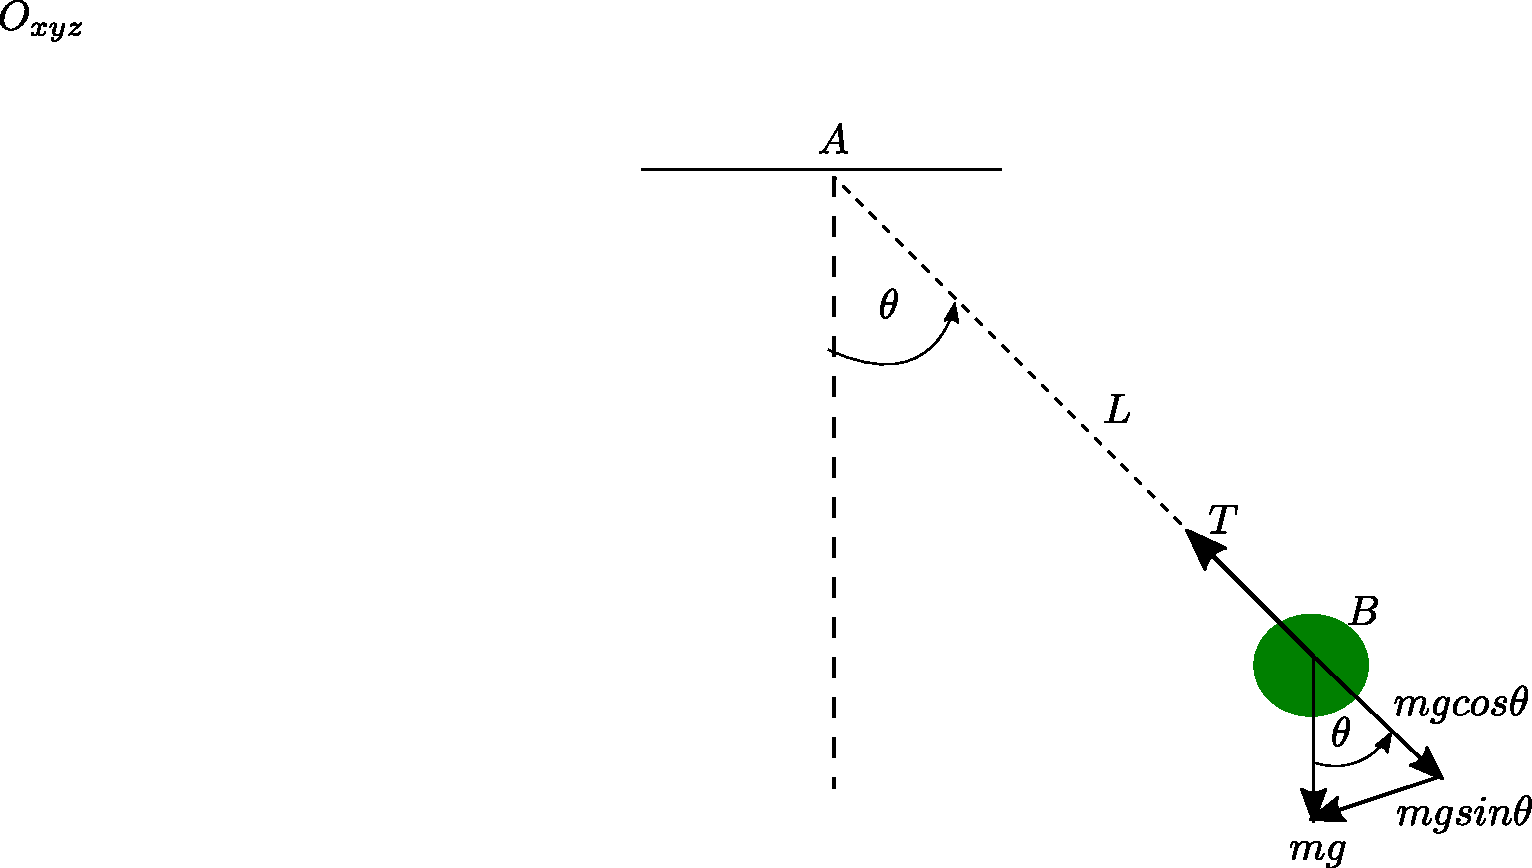
\includegraphics[width=0.4\linewidth]{Bilder/17_PendulumExercise_FBD_Bob.pdf}
	\caption{FBD for pendulum BOB}
	\label{fig_0_ch_4_PendulumProblem_FBD_BOB}
\end{figure}
The pendulums BOB experiences tension T from the link, this force needs to be taken into consideration.

\begin{figure}[h!]
	\centering
	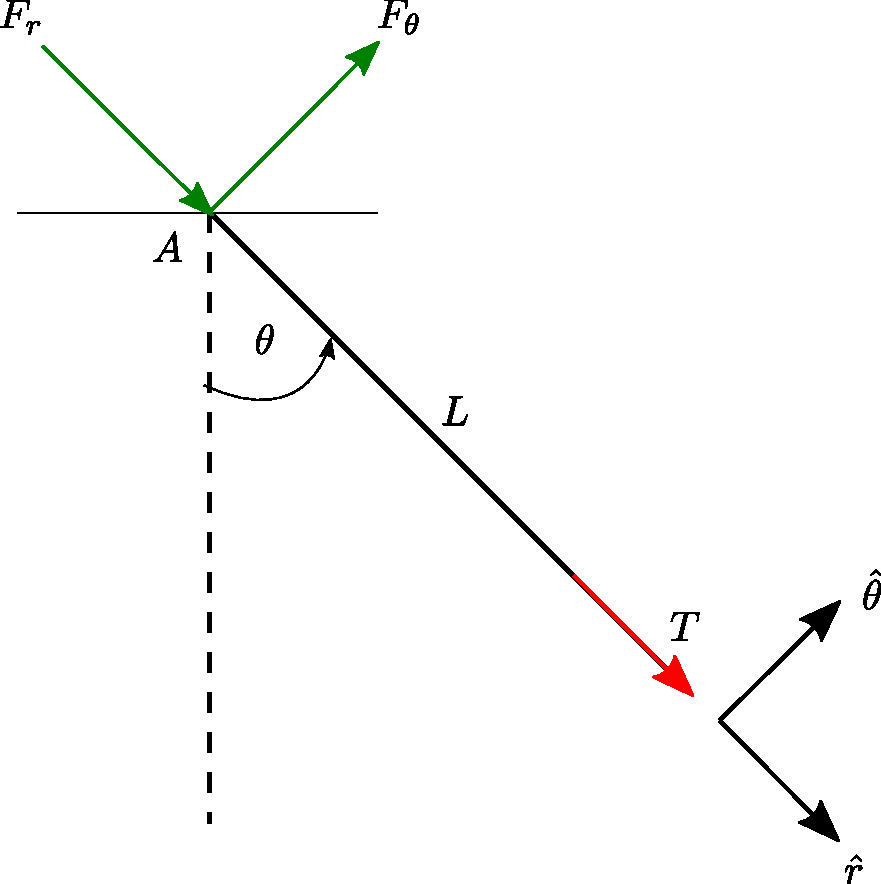
\includegraphics[width=0.4\linewidth]{Bilder/17_PendulumExercise_FBD_Rod.pdf}
	\caption{FBD for pendulum Link}
	\label{fig_0_ch_4_PendulumProblem_FBD_Link}
\end{figure}

The same tension T is experienced by the link in the opposite direction, this force needs to be taken into consideration. Finally, also the reaction forces from the pivot along the $\hat{r}$ and $\hat{\theta}$ should be considered as well. 

Since in this problem, the only interest is to find EOM on $\hat{\theta}$, consider external moments acting about A:
\begin{itemize}
	\item moment due to $mgsin\theta$ as $mglsin\theta$ in the direction opposite to $\hat{\theta}$, acting about $\hat{k}$
	\item moment due to spring force, consider linear with $K_{t}$ as the spring constant: $K_{t}\theta$ in the direction opposite to $\hat{\theta}$, acting about $\hat{k}$
\end{itemize}
there are no other moments produced at point A.
therefore,
\begin{equation}
	\sum \tau_{A} = -mglsin\theta \hat{k} - K_{t}\theta \hat{k}
\end{equation}

\subsection{Complete EOM}

writing both sides of the EOM

\begin{equation}
	-mglsin\theta \hat{k} - K_{t}\theta \hat{k} = \frac{d}{dt}\left(m L^{2} \dot{\theta} \hat{k}\right)
\end{equation}
solving the above equation for $\ddot{\theta}$,
\begin{equation}
	\ddot{\theta} = \frac{-K_{t}\theta - mglsin\theta}{m l^{2}}
\end{equation}

\section{Exercise 2 - self solved}

Consider 1D rotation and 1D translating object as shown in figure \ref{fig_0_ch_4_Ex2}.
\begin{figure}[h!]
	\centering
	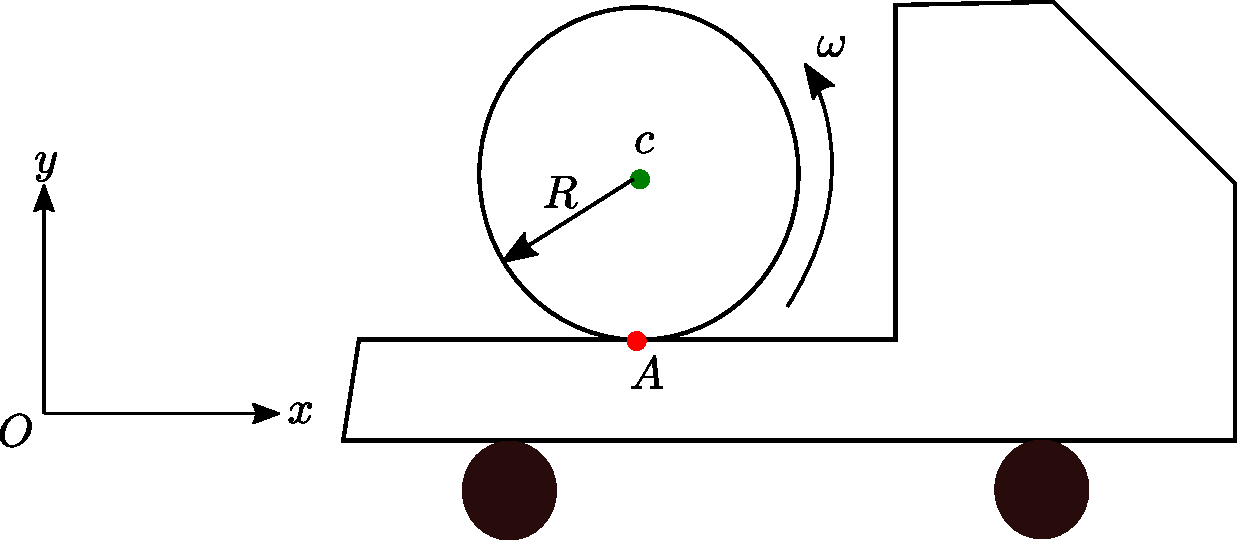
\includegraphics[width=0.5\linewidth]{Bilder/18_TruckNRollProblem.pdf}
	\caption{FBD for pendulum Link}
	\label{fig_0_ch_4_Ex2}
\end{figure}

\subsection{Choosing coordinates}

As this problem is a 1D rotation and 1D translating problem, polar coordinates would suit best for this problem. Choosing $\hat{r}$ positive along the trucks forward motion and $\hat{\theta}$ positive CCW to cylinders roll. Note that the cylinder will move only when the truck is either accelerating or decelerating.

\subsection{DOF}

There are only two possible motions for the cylinder translation $r$ and rotation $\theta$, there will be 2 EOMs. Since this is a rotation problem, equation can be formed of the form
\begin{equation}
\sum \tau_{ext} = \frac{d}{dt}h_{B/A}
\end{equation}

\subsection{Determining angular momentum}

The focus is only on the cylinder, using polar coordinates, the velocity of point A is to be determined. Here the cylinder can only roll about G, therefore, point A is considered as a point fixed w.r.t to a translating point G. using the velocity equation
\begin{equation}
	v_{A/O} = \dot{r}\hat{r} + r \dot{\theta} \hat{\theta}
\end{equation}
where $\dot{r}$ is the translating velocity of point G. 

\begin{equation}
	p_{A/O} = m v_{A/O} = m \left(\dot{r}\hat{r} + r \dot{\theta} \hat{\theta}\right)
\end{equation}

further angular momentum about G
\begin{equation}
	h_{A/G} = r_{A/G} \times p_{A/O} = R \hat{r} \times  m \left(\dot{r}\hat{r} + r \dot{\theta} \hat{\theta}\right)
\end{equation}

As there in this case A is translating w.r.t some fixed frame, torque equation of the following form needs to be considered
\begin{equation}
\sum \tau_{ext} = \frac{d}{dt}h_{A/G} + \frac{d}{dt}v_{G/O} \times p_{A/O}
\end{equation}

\subsection{Determining external moments}

Consider the case when the truck is decelerating, there is a moment produced by the frictional forces about G, which is expressed as
\begin{equation}
	\sum \tau_{G} = -f_{f}R \hat{k}
\end{equation}

\subsection{Finishing EOM}

\begin{align*}
	-f_{f}R \hat{k} &= \frac{d}{dt} \left[R \hat{r} \times  m \left(\dot{r}\hat{r} + R \dot{\theta} \hat{\theta}\right)\right] + \frac{d}{dt} \left(\dot{r}\hat{r}\right) \times m \left(\dot{r}\hat{r} + R \dot{\theta} \hat{\theta}\right) \\
	-f_{f}R \hat{k} &= m R^{2} \dot{\theta} \hat{k} + \left( \ddot{r}\hat{r} + \dot{r}\dot{\theta}\hat{\theta} \right) \times m \left(\dot{r}\hat{r} + R \dot{\theta} \hat{\theta}\right) \\
	-f_{f}R \hat{k} &= m R^{2} \dot{\theta} \hat{k} + \ddot{r}R\dot{\theta}\hat{k} - \dot{r}^{2}\dot{\theta} \hat{k}
\end{align*}
Solving the above for $\ddot{r}$:
\begin{equation}
	\ddot{r} = \frac{\dot{r}^{2}\dot{\theta} - m R^{2} \dot{\theta} -f_{f}R}{R\dot{\theta}}
\end{equation}


\section{Exercise 3}

Consider a translation problem as shown in figure \ref{Fig_0_ch_4_Ex3}.
\begin{figure}[h!]
	\centering
	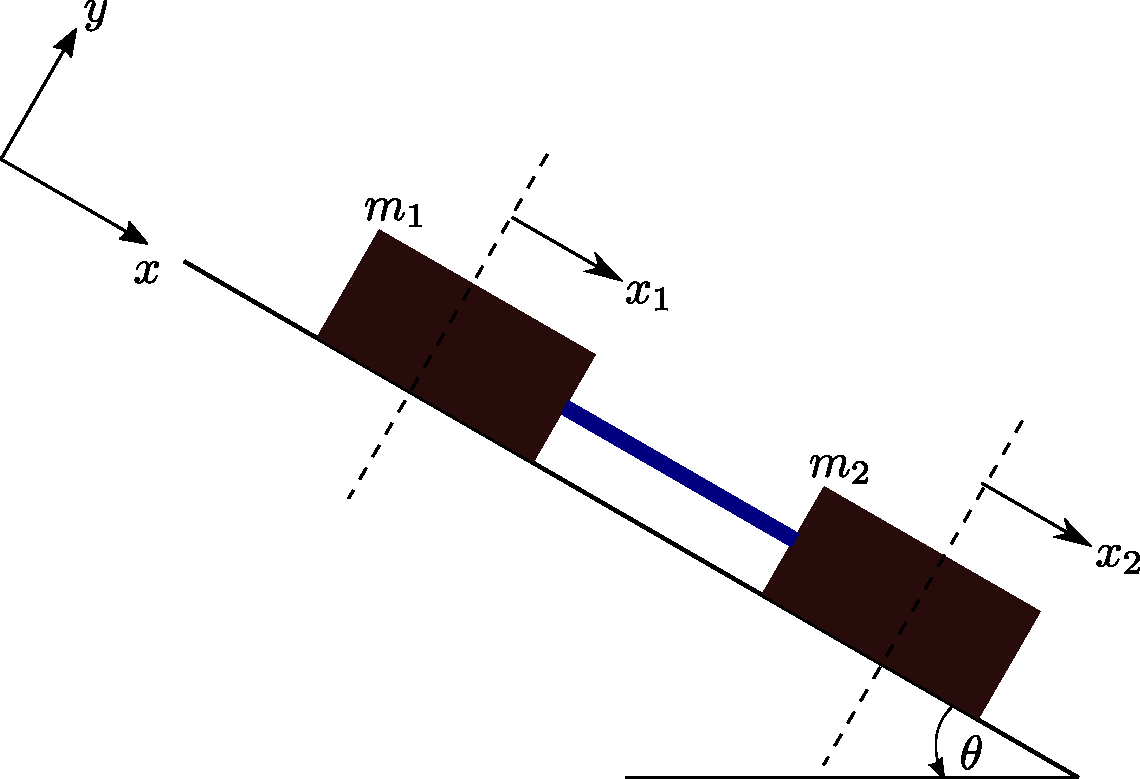
\includegraphics[width=0.5\linewidth]{Bilder/19_TwoMassesRodProblem.pdf}
	\caption{Two sliding masses}
	\label{Fig_0_ch_4_Ex3}
\end{figure}

\subsection{Choosing coordinates}

There are two translating coordinates in this system from the 2 mass, choosing Cartesian coordinate system as shown in figure \ref{Fig_0_ch_4_Ex3}.

\subsection{DOF}
consider constraints
\begin{itemize}
	\item $y_{1} = y_{2} = 0$
	\item $z_{1} = z_{2} = 0$
	\item $\omega_{x1} = \omega_{y1} = \omega_{z1} = \omega_{x2} = \omega_{y2} = \omega_{z2} = 0$
\end{itemize} 

When in Cartesian coordinates, the following formula for DOF can be used
\begin{equation}
	DOF = 6m + 3n - C
\end{equation}
where $m$ is the number of bodies, $n$ is the number of particles (have only 3 translation DOF) and $C$ is the number of constraints. In our case, there 10 constraints as listed above along with another constraint due to \textbf{\textit{Holonomic Constraint}} between the two bodies connected though a link such that $x_{1} = x_{2}$. Therefore, allowing for only one DOF. Because of this Holonomic Constraint, only one EOM is possible for this system.

\subsection{Determining external forces on the system}

Consider figures \ref{Fig_0_ch_4_Ex3_FBD1}\ref{Fig_0_ch_4_Ex3_FBD2} which shows the FBDs for the two bodies.
\newpage
\begin{figure}[h!]
	\centering
	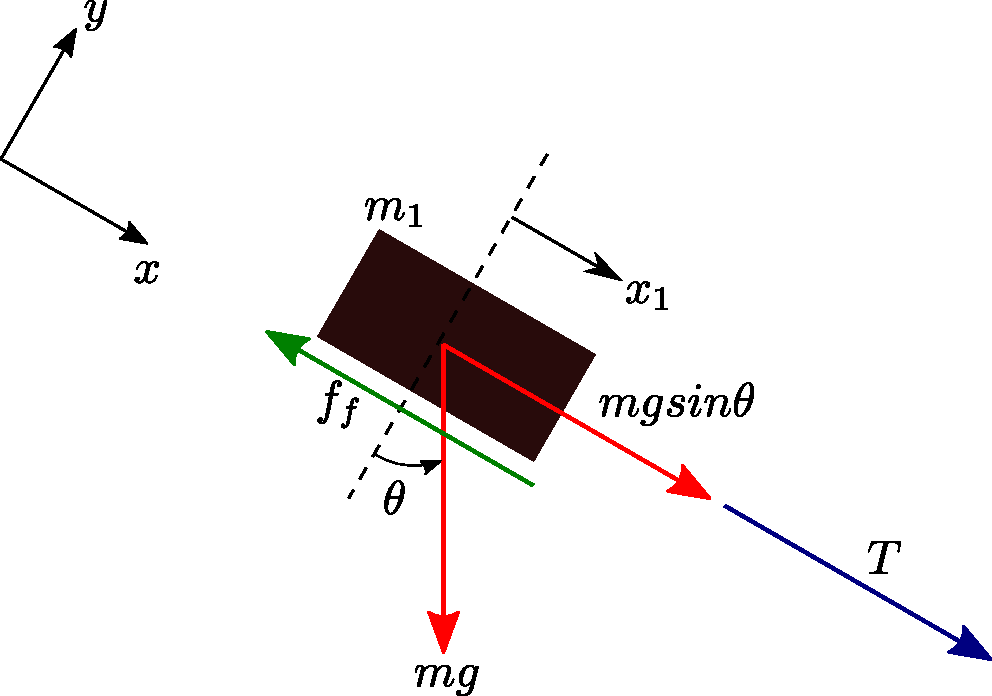
\includegraphics[width=0.5\linewidth]{Bilder/19_TwoMassesRodProblem_FBD_M1.pdf}
	\caption{FBD mass 1}
	\label{Fig_0_ch_4_Ex3_FBD1}
\end{figure}
\begin{figure}[h!]
	\centering
	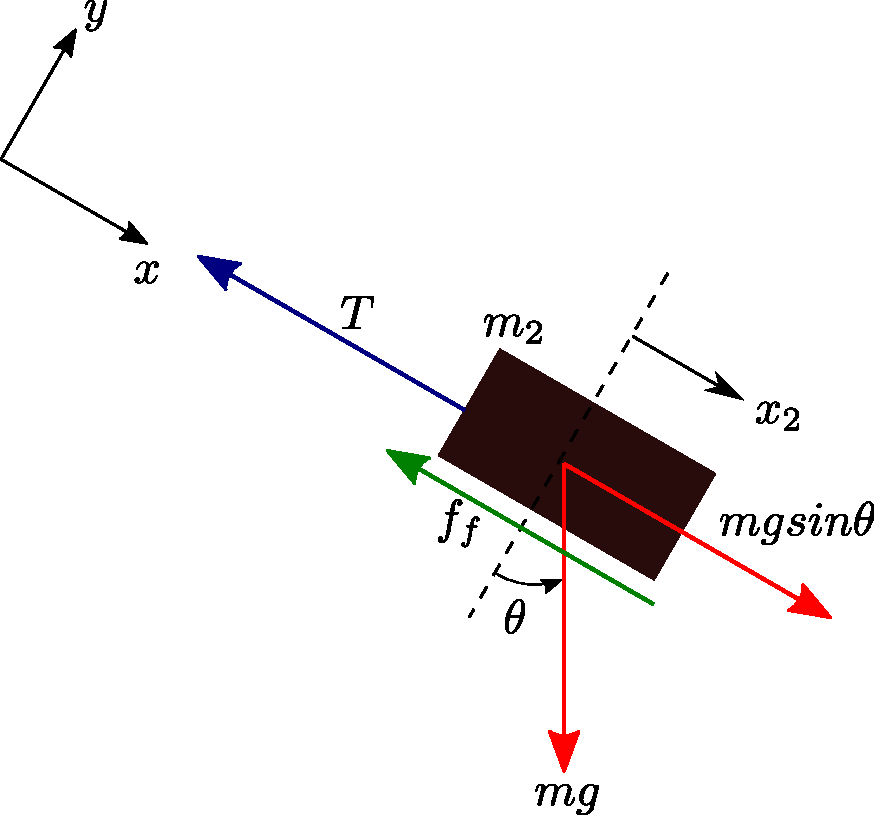
\includegraphics[width=0.5\linewidth]{Bilder/19_TwoMassesRodProblem_FBD_M2.pdf}
	\caption{FBD mass 2}
	\label{Fig_0_ch_4_Ex3_FBD2}
\end{figure}

Since $x_{1} = x_{2}$, consider mass 1 for finding the EOM along x:
\begin{equation}
	\sum F_{x1} = T + mgsin\theta - \mu mg cos\theta
\end{equation}

\subsection{Determining accelerations along x}

There are no rotations in this problem, there is only one component for acceleration along $x$ as $\ddot{x} = \ddot{x}_{1} = \ddot{x}_{2}$. Therefore, only absolute velocity term and no relative velocity terms and terms due to time differentiation of unit vectors.

\subsection{Finishing EOM}

\begin{equation}
	T + mgsin\theta - \mu mg cos\theta = m \ddot{x}_{1}
\end{equation}
solving for $\ddot{x}_{1}$
\begin{equation}
	\ddot{x}_{1} = \frac{1}{m}\left(T + mgsin\theta - \mu mg cos\theta\right)
\end{equation}

\section{Exercise 4}

Consider figure \ref{fig_0_ch_4_twoMassSuspension}.
\begin{figure}[h!]
	\centering
	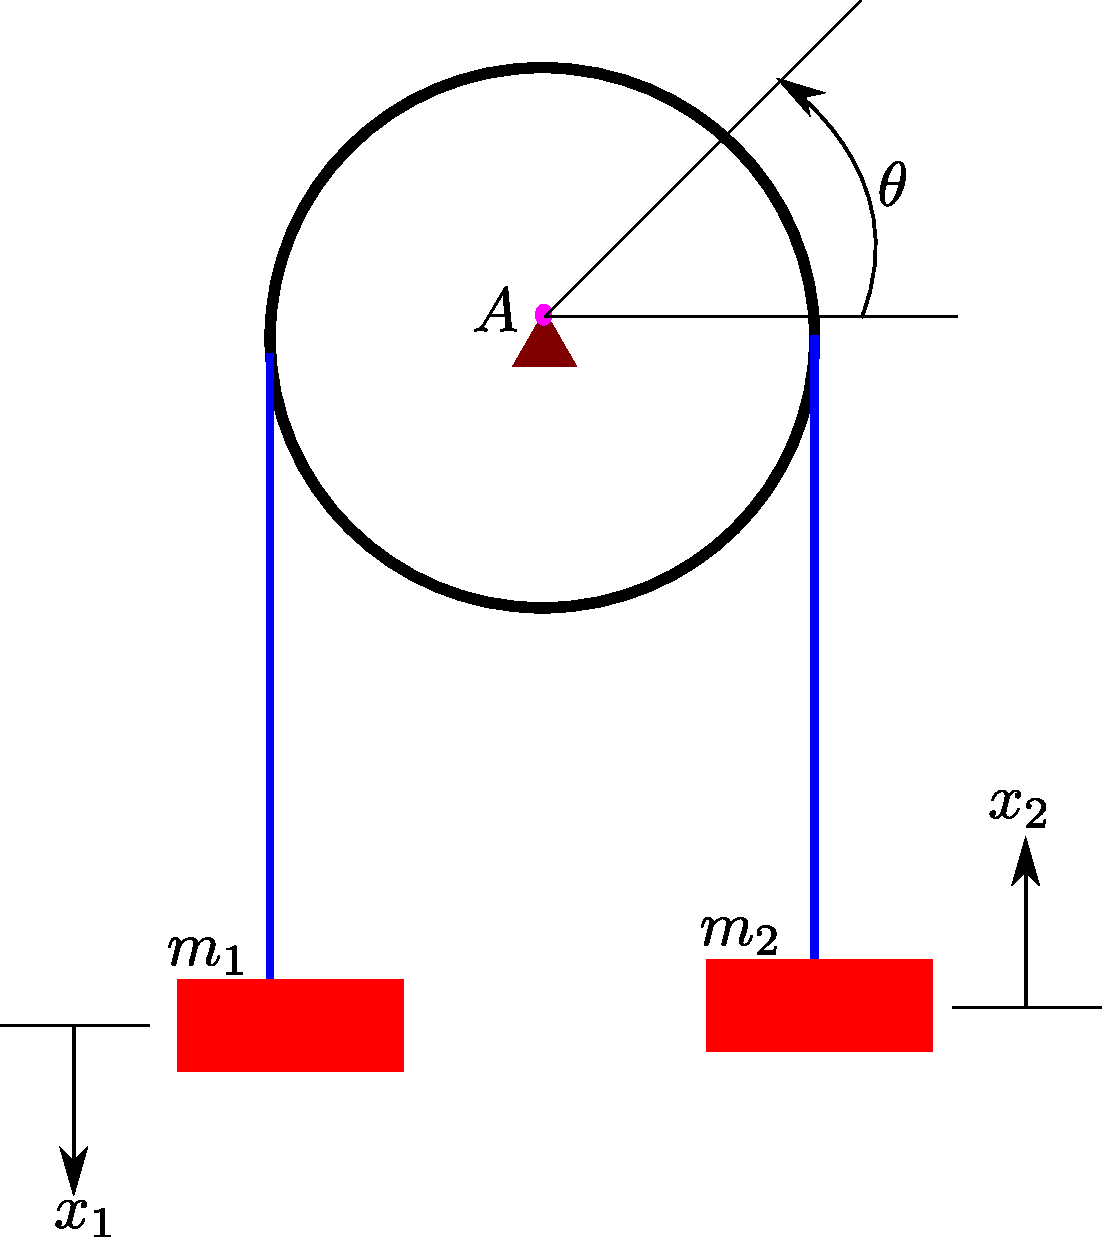
\includegraphics[width=0.5\linewidth]{Bilder/25_TwoMassSuspension.pdf}
	\caption{Two mass suspension system}
	\label{fig_0_ch_4_twoMassSuspension}
\end{figure}

\subsection{Coordinates}
Coordinates are chosen in Cartesian as shown in figure \ref{fig_0_ch_4_twoMassSuspension}. 

\subsection{DOF}
Using the formula $DOF = 6\cdot m + 3 \cdot n - C$, there are 3 masses, no particles. Consider constraints
\begin{enumerate}
	\item $x_{1} = z_{1} = y_{1} = z_{2} = y_{2} = z_{3} = y_{3} = 0$
	\item $M_{x1} = M_{y1} = M_{x2} = M_{y2} = M_{z2} = M_{x3} = M_{y3} = M_{z3}  = 0$
\end{enumerate}
Additionally, there is a holonomic constraint such that, $x_{1} = x_{2}$. Therefore, leading to 2 DOFs. The EOM should be formed as
\begin{align}
	\sum F_{ext} &= m a_{x1/O} \quad or \quad \sum F_{ext} = m a_{x2/O} \\
	\sum M_{ext} &= \frac{d}{dt}h_{A/O}
\end{align}

\subsection{External forces}

Consider the FBDs of the two masses as shown in the figure \ref{fig_0_ch_4_twoMassSuspension_FBD_masses}.
\begin{figure}[h!]
	\centering
	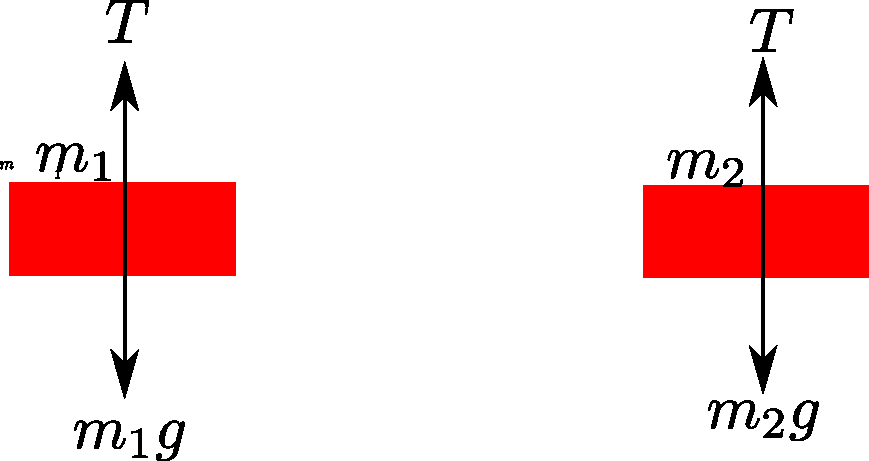
\includegraphics[width=0.5\linewidth]{Bilder/25_TwoMassSuspension_FBD_Masses.pdf}
	\caption{FBD of two mass}
	\label{fig_0_ch_4_twoMassSuspension_FBD_masses}
\end{figure}

Because of all the constraints, the possible acceleration is as follows
\begin{equation}
	\sum F_{x1} = m a_{x1/O} = m \ddot{x1} \quad or \quad \sum F_{x2} = m a_{x2/O} = m \ddot{x2}
\end{equation}

\subsection{External moments}

Consider the FBD of the wheel as shown in figure \ref{fig_0_ch_4_twoMassSuspension_FBD_Wheel}.
\begin{figure}[h!]
\centering
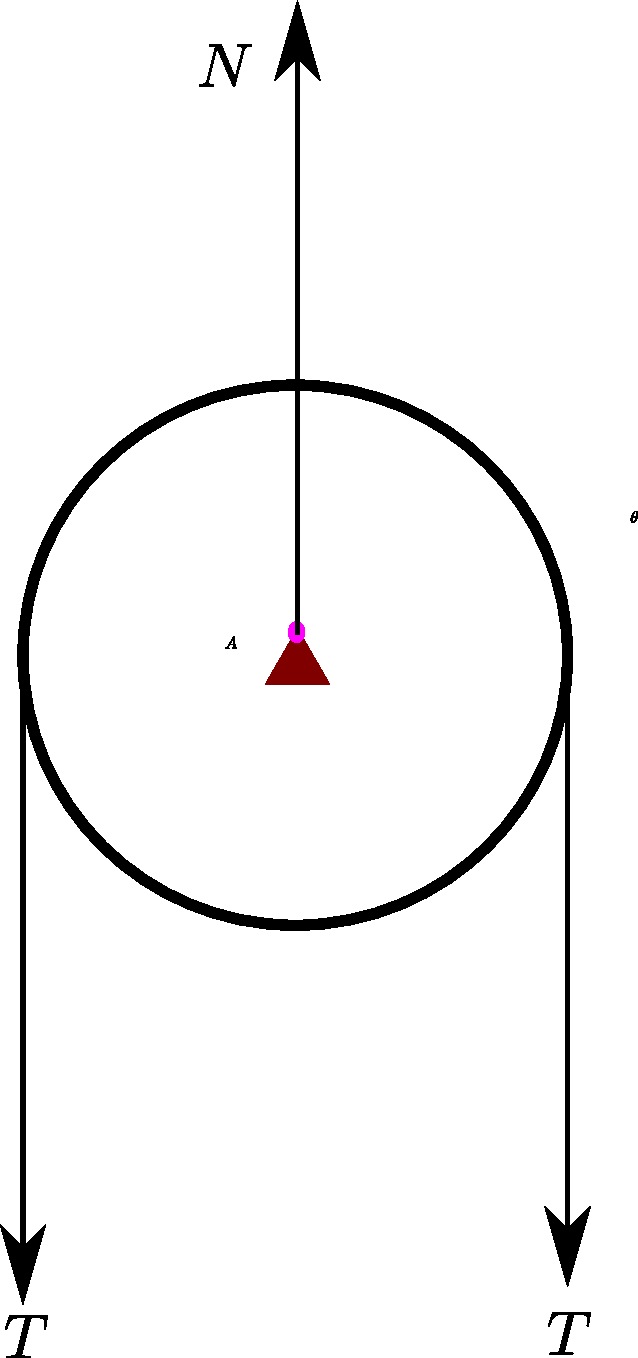
\includegraphics[width=0.2\linewidth]{Bilder/25_TwoMassSuspension_FBD_Wheel.pdf}
\caption{FBD of wheel}
\label{fig_0_ch_4_twoMassSuspension_FBD_Wheel}
\end{figure}

If the masses $m_{1} = m_{2}$ is considered, then the tension on the string on both sides will be the same, therefore, canceling out the moments by $T$ about A. If in case $m_{1} \neq m_{2}$, then the moment produced will be greater on the side of higher mass, this will lead to the heavier mass hitting the ground or unless it is stopped using a stopper. However, lets consider that $m_{1} \neq m_{2}$ so that the problem can be solved for $\ddot{\theta}$ and $\ddot{x}$.

External moments acting about A due to $m_{1} \neq m_{2}$ can be expressed as
\begin{equation}
	\sum \tau_{/A} = \left(m_{1}gR - m_{2}gR\right)\hat{k}_{1}
\end{equation}

However, this is not completely true, as in Newtonian Mechanics, string tension $T$ is considered as internal to the system. So for the system as a whole, in this problem, there are no external moments. In this problem, it can be considered that there is a moment applied at A, which is equal to the the equation mention above.

\subsection{Finishing the EOMs}

Consider the wheel, the angular momentum about A is expressed as
\begin{align*}
	h_{A/O} &= r_{m{1}/A} \times  p_{m1/O} + r_{m{2}/A} \times p_{m2/O} \\
			&= R\hat{j}_{1} \times m_{1}\dot{x}_{1} \hat{i}_{2} + R\hat{j}_{1} \times m_{2}\dot{x}_{2} \hat{i}_{3} \\
			&= - m_{1} R \dot{x}_{1} \hat{k}_{1} - m_{2} R \dot{x}_{2} \hat{k}_{1} \\
			&= - \left(m_{1} + m_{2}\right) R \dot{x} \hat{k}_{1}
\end{align*}
in the above equation $\dot{x}_{1} = \dot{x}_{1} = \dot{x}$ due to the constraint the non-holonomic constraint, which results due to the holonomic constraint $x_{1} = x_{2}$
\begin{align*}
	\left(m_{1}gR - m_{2}gR\right)\hat{k}_{1} &= - \frac{d}{dt} \left(m_{1} + m_{2}\right) R \dot{x} \hat{k}_{1} \\
											&= - \left(m_{1} + m_{2}\right) R\ddot{x}
\end{align*}
solving the above equation for $\ddot{x}$:
\begin{equation}
	\ddot{x} = - \frac{\left g (m_{1} - m_{2}R\right)}{\left(m_{1} + m_{2}\right)}
\end{equation}












